% Ch2 slides: mass balance on a fluid element - (A) out, (B) in, (C) accumulation inside
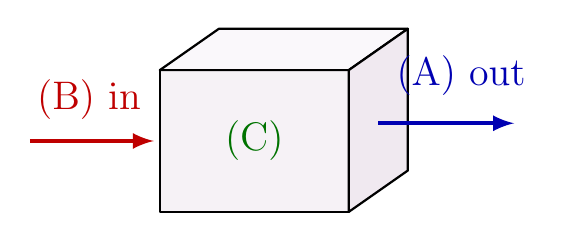
\begin{tikzpicture}[scale=1.5, >=latex, line join=round]
  \definecolor{dpurple}{HTML}{68246D}
  \draw[thick, fill=dpurple!6] (0,0) rectangle (1.6,1.2);
  \draw[thick, fill=dpurple!3] (0,1.2) -- (0.5,1.55) -- (2.1,1.55) -- (1.6,1.2) -- cycle;
  \draw[thick, fill=dpurple!10] (1.6,0) -- (2.1,0.35) -- (2.1,1.55) -- (1.6,1.2) -- cycle;
  \draw[->, ultra thick, red!75!black] (-1.1,0.6) -- (-0.05,0.6);
  \node[red!75!black, font=\Large] at (-0.6,0.95) {(B) in};
  \draw[->, ultra thick, blue!70!black] (1.85,0.75) -- (3.0,0.75);
  \node[blue!70!black, font=\Large] at (2.55,1.15) {(A) out};
  \node[green!45!black, font=\Large] at (0.8,0.6) {(C)};
\end{tikzpicture}
